\section{Case study: effective rank as evidence for superficial post-training}
\label{sec:timber}

\citet{wu2025timber} compare released base and instruct models (Llama~3 and
Qwen3) through the entropy effective rank of each weight matrix. They report
that $\entropyrank(W_{\text{base}})$ and $\entropyrank(W_{\text{instruct}})$
are nearly identical for every layer, read this as weight-level evidence that
post-training is superficial, and report $\entropyrank(\dW)$ at around 85\% of
full rank. They then edit instruct models by keeping the top
$K = \lceil \entropyrank(\dW) \rceil$ singular directions of $\dW$ and scaling
the rest by $\lambda \in [0, 1)$, which improves pass@$k$ on their benchmarks.
We test the measurement and the cutoff with the baselines of
\S\ref{sec:background}.

\paragraph{Reproduction.} On Qwen3-0.6B and Qwen3-8B, two of the pairs in
their study, we measure $\entropyrank(\dW)$ at 83\% of full rank for both,
consistent with their figure.

\subsection{An unchanged effective rank is what any small update produces}

\begin{figure}[t]
\begin{center}
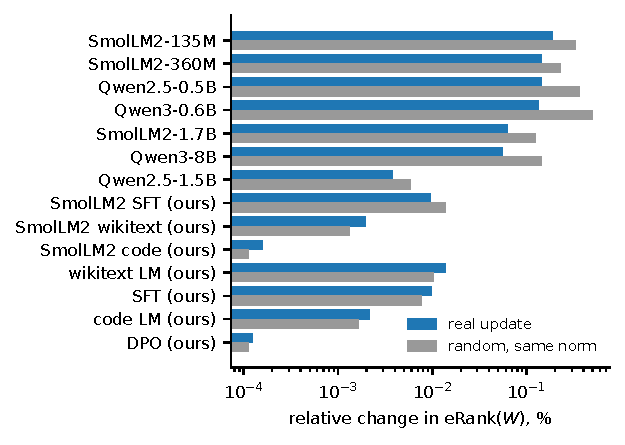
\includegraphics[width=0.62\linewidth]{figures/erank_perturbation.pdf}
\end{center}
\caption{Relative change in the entropy effective rank of the full weight
matrix $W$ caused by the real update (blue) and by a Gaussian perturbation
with the same Frobenius norm (grey), averaged over matrices. Log scale. Every
change, real or random, is below 0.5\%.}
\label{fig:erank}
\end{figure}

For every matrix we compare the change in $\entropyrank(W)$ caused by the real
update with the change caused by a random perturbation of the same norm
(Figure~\ref{fig:erank}; Table~\ref{tab:erankw} in the appendix). The update
is 0.05--1.4\% of $\|W\|_F$ for our runs and 1.2--12.6\% for the released
models. Across all fourteen cases the effective rank of $W$ moves by less than
0.5\%, and the random perturbation moves it by a similar amount: for Qwen3-8B,
0.06\% for the real update and 0.14\% for the random one; for our SFT run,
0.010\% and 0.008\%. This is the behaviour Weyl's inequality predicts, and it
means an unchanged effective rank of $W$ follows from the update being small.
It holds equally for our fine-tunes on Wikipedia and on code, so it cannot
distinguish superficial post-training from ordinary fine-tuning.

There is one detail in Timber's favour. On the released models the real
update moves the effective rank 1.5--4$\times$ less than a random one of the
same norm, so post-training does change $W$ in a structured way. That only
becomes visible with the random comparison, and it is a statement about
structure, not about superficiality.

\subsection{The effective rank of the update sits near the noise value}

On the update itself, $\entropyrank(\dW)$ is 0.79--0.90 of full rank for the
released pairs against 0.87--0.93 for Gaussian matrices of the same shapes, a
ratio of 1.03--1.14 (Qwen3-8B: 0.83 against 0.91). Stable rank separates the
same updates from noise by 1.6--9.1$\times$ (\S\ref{sec:released}). The
eRank-based cutoff of 83\% of full rank therefore sits close to where a random
matrix would put it.

\subsection{Does the cutoff matter?}
\label{sec:cutoff}

\begin{figure}[t]
\begin{center}
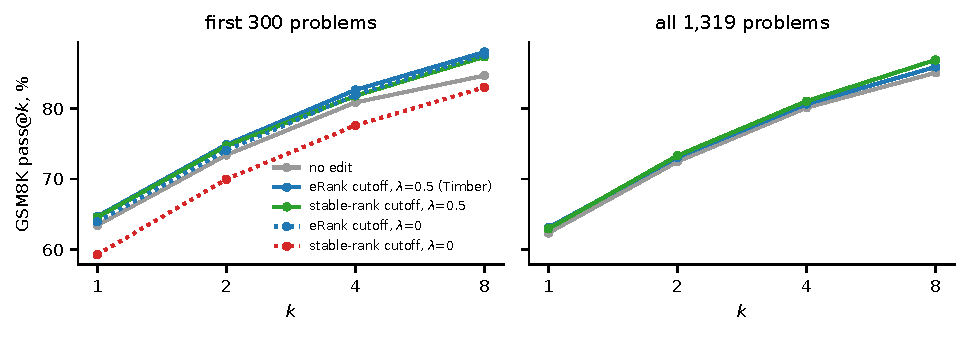
\includegraphics[width=\linewidth]{figures/cutoff_passk.pdf}
\end{center}
\caption{GSM8K pass@$k$ for Qwen3-0.6B (non-thinking mode) edited as in
\citet{wu2025timber}, with their eRank cutoff and with a stable-rank cutoff.
Left: the first 300 test problems, all five variants. Right: all 1{,}319
problems for the unedited model and the two $\lambda=0.5$ variants. Eight
samples per problem, the same sampling seed per problem for every variant.}
\label{fig:cutoff}
\end{figure}

\begin{table}[t]
\caption{Timber's edit on Qwen3-0.6B with two cutoffs, on all 1{,}319 GSM8K
test problems (8 samples each). ``Kept'' is the share of $\dW$'s energy left
unscaled. Differences from the unedited model are in points, with 95\% paired
bootstrap intervals over problems.}
\label{tab:cutoff}
\begin{center}
\small
\begin{tabular}{lccccc}
\toprule
variant & kept & pass@1 & pass@8 & $\Delta$ pass@1 & $\Delta$ pass@8 \\
\midrule
no edit                              & 100\%  & 62.3 & 85.1 & -- & -- \\
eRank cutoff, $\lambda=0.5$ (Timber) & 98.9\% & 63.1 & 85.9 & $+0.8$ ($-0.0$, $+1.6$) & $+0.8$ ($-0.6$, $+2.3$) \\
stable cutoff, $\lambda=0.5$         & 41.4\% & 62.9 & 86.9 & $+0.6$ ($-0.5$, $+1.7$) & $+1.8$ ($+0.2$, $+3.5$) \\
\bottomrule
\end{tabular}
\end{center}
\end{table}

On Qwen3-0.6B the eRank cutoff keeps 83\% of the directions and 98.9\% of the
update's energy, so Timber's edit changes about 1\% of the update. A cutoff at
$\lceil r \cdot \stablerank(\dW) \rceil$ keeps 12\% of the directions and
41\% of the energy. We apply the same edit with both cutoffs, at $\lambda = 0$
(their Timber-L) and $\lambda = 0.5$, and score pass@$k$ \citep{chen2021codex}
on GSM8K \citep{cobbe2021gsm8k} in non-thinking mode with the sampling
settings recommended for it (temperature 0.7, top-$p$ 0.8, top-$k$ 20).
\citet{wu2025timber} did not report GSM8K, so this is a test of the cutoff
rather than a reproduction of their table.

Three findings (Figure~\ref{fig:cutoff}, Table~\ref{tab:cutoff}):

\begin{itemize}
  \item \textbf{Removing the tail hurts.} On the first 300 problems, the
  stable-rank cutoff at $\lambda = 0$ lowers pass@1 by 4.2 points (interval
  $-6.9$ to $-1.4$), and the share of samples that reach a final answer falls
  from 96.5\% to 90.6\%. The noise-like 59\% of the update's energy matters to
  the model, which agrees with the finding of \citet{ping2024deltacome} that
  truncating $\dW$ to low rank degrades fine-tuned models.
  \item \textbf{Halving it does not.} At $\lambda = 0.5$ the two cutoffs give
  the same result. Directly compared on all 1{,}319 problems, the stable-rank
  variant differs from Timber's by $-0.2$ points of pass@1 ($-1.2$ to
  $+0.9$) and $+1.0$ of pass@8 ($-0.6$ to $+2.5$), although it scales about
  40$\times$ more of the update. The eRank boundary is not special.
  \item \textbf{The benefit is small on this benchmark.} On the first 300
  problems Timber's edit raised pass@8 by 3.3 points ($+0.3$ to $+6.3$), the
  pattern their paper reports. On the full set the gain is $+0.8$ ($-0.6$ to
  $+2.3$), and on the 1{,}019 problems outside the first 300 it is $+0.1$
  ($-1.6$ to $+1.7$). The only interval in Table~\ref{tab:cutoff} that clears
  zero, pass@8 for the stable-rank variant, does so by little among six
  comparisons, and we do not read anything into it.
\end{itemize}

None of this contradicts the gains \citet{wu2025timber} report on other
benchmarks, which we did not test. It does say that the effective rank of
$\dW$ is not what makes the edit work, and that pass@$k$ gains measured on a
few hundred problems can shrink substantially on the full set.
